\begin{figure}[htbp]
\centering
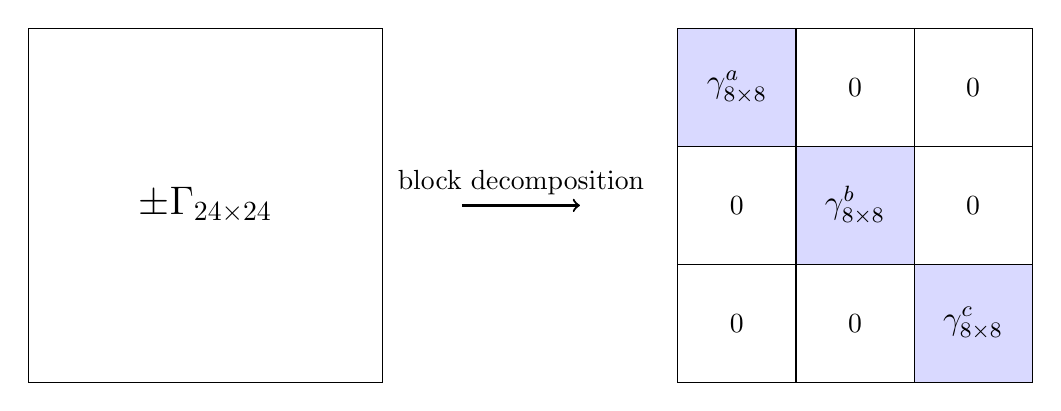
\begin{tikzpicture}[
    matrixbox/.style={
        draw,
        minimum width=4.5cm,
        minimum height=4.5cm
    },
    blocklabel/.style={font=\large}
]

% Original matrix
\node[matrixbox, font=\Large] (full) at (0,0)
    {$\pm\Gamma_{24\times24}$};

% Arrow
\draw[->, thick] ([xshift=1cm]full.east) -- ++(1.5,0)
    node[midway, above] {block decomposition};

% Block-diagonal matrix
\begin{scope}[shift={(6, -2.25)}]
    % Highlight diagonal blocks
    \fill[blue!15] (0,3) rectangle (1.5,4.5);
    \fill[blue!15] (1.5,1.5) rectangle (3,3);
    \fill[blue!15] (3,0) rectangle (4.5,1.5);

    % Outer box and grid
    \draw (0,0) rectangle (4.5,4.5);
    \draw (1.5,0) -- (1.5,4.5);
    \draw (3,0) -- (3,4.5);
    \draw (0,1.5) -- (4.5,1.5);
    \draw (0,3) -- (4.5,3);

    % Diagonal blocks
    \node[blocklabel] at (0.75,3.75) {$\gamma^a_{8\times8}$};
    \node[blocklabel] at (2.25,2.25) {$\gamma^b_{8\times8}$};
    \node[blocklabel] at (3.75,0.75) {$\gamma^c_{8\times8}$};

    % Off-diagonal blocks
    \node at (2.25,3.75) {$0$};
    \node at (3.75,3.75) {$0$};
    \node at (0.75,2.25) {$0$};
    \node at (3.75,2.25) {$0$};
    \node at (0.75,0.75) {$0$};
    \node at (2.25,0.75) {$0$};
\end{scope}

\end{tikzpicture}
\caption{Schematic decomposition of a projected local Majorana operator in a
\(24\)-dimensional energy sector. The sector separates into three independent
\(8\times8\) blocks, labelled \(a\), \(b\), and \(c\), with one effective
Majorana block acting within each subspace.}
\label{fig:24x24maj}
\end{figure}
